\documentclass{article}
\usepackage{graphicx}
\usepackage{subcaption}
\usepackage[utf8]{inputenc}
\usepackage{biblatex}
\usepackage{amsmath}

\addbibresource{references.bib}

\title{Exploration of Alternative Cryptocurrencies in Relation to Electricity Consumption and Climatic Impact}
\author{Taylor Giles, Matthew Broadbent, Srdjan Bozin}
\date{May 2022}

% Remove section numbering
\setcounter{secnumdepth}{0}

\begin{document}

\maketitle

\section{Introduction}

In this report, we expand upon the assessment performed by Goodkind et al. of the environmental and economic damages caused by cryptocurrency mining in their paper, "Cryptodamages: Monetary value estimates of the air pollution and human health impacts of cryptocurrency mining'' \cite{goodkind}.

Goodkind and colleagues analyzed damages caused by Proof-of-Work (POW) coins - specifically Bitcoin, Ethereum, Litecoin, and Monero. Our objective is to perform similar analyses on Proof-of-Stake (POS) and other alternative coins to determine the magnitude of potential benefit to be gained from using "greener" coins. 

Proof-of-Work and Proof-of-Stake are the two major consensus algorithms for blockchains. To achieve consensus in a POW blockchain, virtual miners race to be the first to solve a complex math problem. The first to do so updates the blockchain with the recent verified transactions and is rewarded cryptocurrency by the network. In a POS blockchain, network participants may similarly validate the recent transactions and receive a reward in the cryptocurrency. The difference from POW, though, is that participants may stake their cryptocurrency in the network for a chance to be selected to validate the blockchain and receive the reward. The chance you are selected is proportional to how much you stake \cite{posscale}. 

POS blockchains generally require far less energy consumption than POW because they do not involve these very complex and expensive calculations.

In addition to this, the positive feedback loop of increasing computational power dedicated towards POW systems, which is described in the paper by Goodkind et al. \cite{goodkind}, does not exist in POS systems as the limiting factor is not one's computational power but rather one's staking potential, which carries with it an opportunity cost. Despite these trade-offs, it seems apparent that POS-based systems could revolutionize cryptocurrencies by solving the scalability problem.


\section{Coins}
For this paper, we decided to focus primarily on POS coins, as they typically result in far less energy demand, yet the model is still popular enough that we would be able to find some reliable data.

The cryptocurrencies we selected to examine include:
\begin{itemize}
    \item \textbf{Nano}: Nano was an interesting choice because it markets itself as a far superior version to BitCoin given its feeless transactions, faster speeds, and astronomically lower energy requirements.
    \item \textbf{Cardano}: With a price of approximately \$1, Cardano stood out as a coin with a high worth as a cryptocurrency. This made it seem more comparable to a mainstream cryptocurrency.
    \item \textbf{Algorand}: Created by an MIT cryptography professor, this coin aims to solve the cryptocurrency trilemma with an emphasis on sustainability.
    \item \textbf{Solana}: A very innovative and popular coin that created the concept of Proof-of-History, enabling it to have extreme speed and a very high transaction rate.
    \item \textbf{Hedera}: Hedera HBAR is powered by the Hedera Hashgraph, an alternative to traditional blockchain-based systems which promises to ``lead the way for the future of public ledgers.'' \cite{hbar}
    \item \textbf{SolarCoin}: Although not analyzed in this report, we felt that SolarCoin was worth mentioning due to its unique approach of distributing coins to producers of solar energy.
\end{itemize}

\subsection{Nano}

Nano is a decentralized digital currency, aiming to do what BitCoin does, but faster, feeless, and requiring magnitudes less energy.

Nano is unique in a few ways. First of all, there is not one blockchain- each user account has their own blockchain representing transactions involving that account. The network uses an Open-Representative-Voting system, similar to a traditional POS, however being selected as a validator does not offer any internal incentives - you are not rewarded any currency. This helps the network remain decentralized (and by extension secure), as offering cryptocurrency to those who can already afford to stake their own can lead to increased centralization \cite{orvconsensus}.

Nano has approximately 80,000 transactions per day \cite{nanolooker}, and requires only 0.000112 kWh of energy per transaction \cite{realsimple}.

\subsection{Cardano}

Cardano is built using the Ouroboros protocol, which uses a POS model. Cardano is known for its ability to select a representative with very little bias. This results in a highly secure network, so long as at least 51\% of the network is controlled by honest parties \cite{ouroboros}.

Cardano consumes 0.5479 kWh per transaction \cite{cryptovantage}, and completes approximately 100,000 transactions per day \cite{cardanodatastudio}.

Cardano stands out as much more energy demanding than the other coins highlighted in this paper. This could be because Cardano was the first POS based cryptocurrency to be based on peer-reviewed research, and is provably secure. Granted, it is still 47,000 times less energy intensive than BitCoin \cite{cardanodatastudio}.

\subsection{Algorand}

Algorand dubs itself as the “green blockchain.” Its goal is to solve the crypto trilemma of decentralization, security, and scalability.  From its creation it was made with sustainability in mind and continues to operate at a carbon-negative level, with validation requiring negligible energy \& computational resources. Algorand is currently in a phase of hyper-growth, as it has been adopted by some countries to be the underlying blockchain for their currency and continues to grow in popularity. 

It is able to maintain its green edge by keeping validator influence proportional to validator stake. In a traditional POS system the stakers of the coin reap the rewards, but Algorand uses a Pure Proof-of-Stake (PPOS) system whereby staking gives one influence as a validator, but everyone who holds the coin receives a return \cite{algoppos}.

Algorand validation can be run on a Raspberry PI with high efficiency. We assume that all validators are rational and use a Raspberry PI at full power as their machine of choice. This assumption would imply a power of $P = 7.2[W]$ per validator node. 

If we assume $T = 1000[transactions/sec]$ are processed in by the PPOS system, we can derive the energy spent by each validator for each transaction using the formula:

$E = \frac{P}{T} = \frac{7.2[W]}{1000\frac{[t]}{[s]}}$.

We can convert the units of this using the rate: $[J] = \frac{1}{3600}[Wh]$

$E = \frac{7.2[W]}{1000\frac{[t]}{[s]}} * \frac{1 [Wh]}{3600 [J]} = \frac{7.2[W]}{1000\frac{[t]}{[s]}} * \frac{1 [Wh]}{3600 [Ws]} = 2 * 10^{-6} \frac{[Wh]}{[t]} = 2 \frac{{[\mu}Wh]}{[t]}$.

Now that we have the energy used per validator per transaction we can estimate the entire coin's energy usage per transaction by considering that it has around 4000 validators.

$E_{T} = E * 4000 = 2 \frac{{[\mu}Wh]}{[t} * 4000 = 0.008 \frac{[Wh]}{[t]}$ \cite{algoestimate}

So we can conclude our estimate that Algorand uses about $0.008 [Wh]$ per transaction. 

\subsection{Solana}

Due to its extremely fast processing and inexpensive fees, Solana is the most popular coin examined in this analysis. It is also a POS system, but integrated under the hood of Proof-of-History (POH), which is the secret to its extremely fast validation speed.

While most other blockchains rely on sequential block processing, which can cause delays, POH enables Solana nodes to send in their updates out of order. The protocol requires each validator to keep their own cryptographic clock which enables them to timestamp their updates in a secure and maintainable fashion. This enables requests to be accumulated asynchronously, reducing delays and improving speed \cite{solanaworks}.

The major benefit of the POH system is that validators do not need to communicate amongst each other to ensure that blocks are updated in the right order. Nodes follow a predetermined protocol and are able to work independently, sending timestamped blocks whenever necessary. These blocks can be sorted using their timestamp to reliably and securely recreate the correct sequence. 

\subsection{Hedera}
Hedera (HBAR) is a cryptocurrency build on the Hedera Hashgraph network, which is a decentralized network for consensus and smart contracts based on directed acyclic graphs (DAGs) instead of traditional blockchain technology. Hedera believes that this technology can make global tokenization a reality, and prides itself on the efficiency of the decentralized network \cite{hbar}.

HBAR consumes an approximate $0.00017$ kWh per transaction and can support up to $10,000$ transactions per second, but currently performs at approximately 1 million transactions per day \cite{hbar}.


\subsection{SolarCoin}
SolarCoin is a relatively new coin with very little data available, but we felt that it was important to mention in this report due to its unique approach as a green cryptocurrency. The objective of the SolarCoin project is to make clean energy more desirable by providing incentive in the form of cryptocurrency. Producers of solar energy can ``file a claim to register their solar installation'' and in doing so, make themselves eligible to collect one SolarCoin per MWh of generated solar energy \cite{solarcoin}. At the moment, this is a very small incentive (one SolarCoin is worth under one cent \cite{solarcoin_price}, and one MWh is a large amount of energy), however the concept is valuable within the scope of this report. In theory, SolarCoin could have a net social value greater than 100\%, as energy is produced in the collection of a coin rather than consumed. With the growing popularity of solar energy in the U.S. \cite{solar}, this coin could have a bright future. However, due to the scarcity of data surrounding this coin, it was not analyzed to the same extent as the other coins featured in this report.

\section{Procedure \& Data Collection}
Our analysis aims to broadly assess the viability and potential benefits of several ``green'' cryptocurrencies with regard to environmental impact and ``net social value'' as defined in the paper by Goodkind and colleagues \cite{goodkind}. They define ``net social value'' as the metric by which a cryptocurrency can be evaluated for its total monetary impact on society. The equation they used is as follows: 

\begin{multline*}
\text{net social value} = \text{coin price} - (\text{cost of energy} \\ 
* \text{energy needed per coin}) - \text{ damages caused per coin}
\end{multline*}

For Goodkind and his colleagues, the ``damages per coin'' involved a monetary representation of the climate-related and health-related impacts of the energy generation needed to sustain each of the coins in their study. Unfortunately, the data required to draw conclusions about health-related damages were not available to us, but we were able to estimate climate-related damages by using the Social Cost of Carbon (SCC). The SCC is a government-established metric which gives a monetary value to the societal damages caused by carbon dioxide emissions, and is currently set at \$51 per ton of $\text{CO}_2$ \cite{scc}.

We decided to focus our analysis on the United States, since data for that region is most readily available and accessible. First, we collected statistics about energy production. Specifically, we handled data for the generation of electricity \cite{elec_gen}, the cost of electricity \cite{elec_cost}, and $\text{CO}_2$ emissions caused by electricity generation \cite{co2} in the U.S. from 2000 - 2022 (Fig. \ref{fig:us_data}). With this data, we were able to calculate the amount of carbon dioxide produced per kWh of generated electricity over time (Fig. \ref{fig:us_data}).

\begin{figure}[h!]
    \centering
    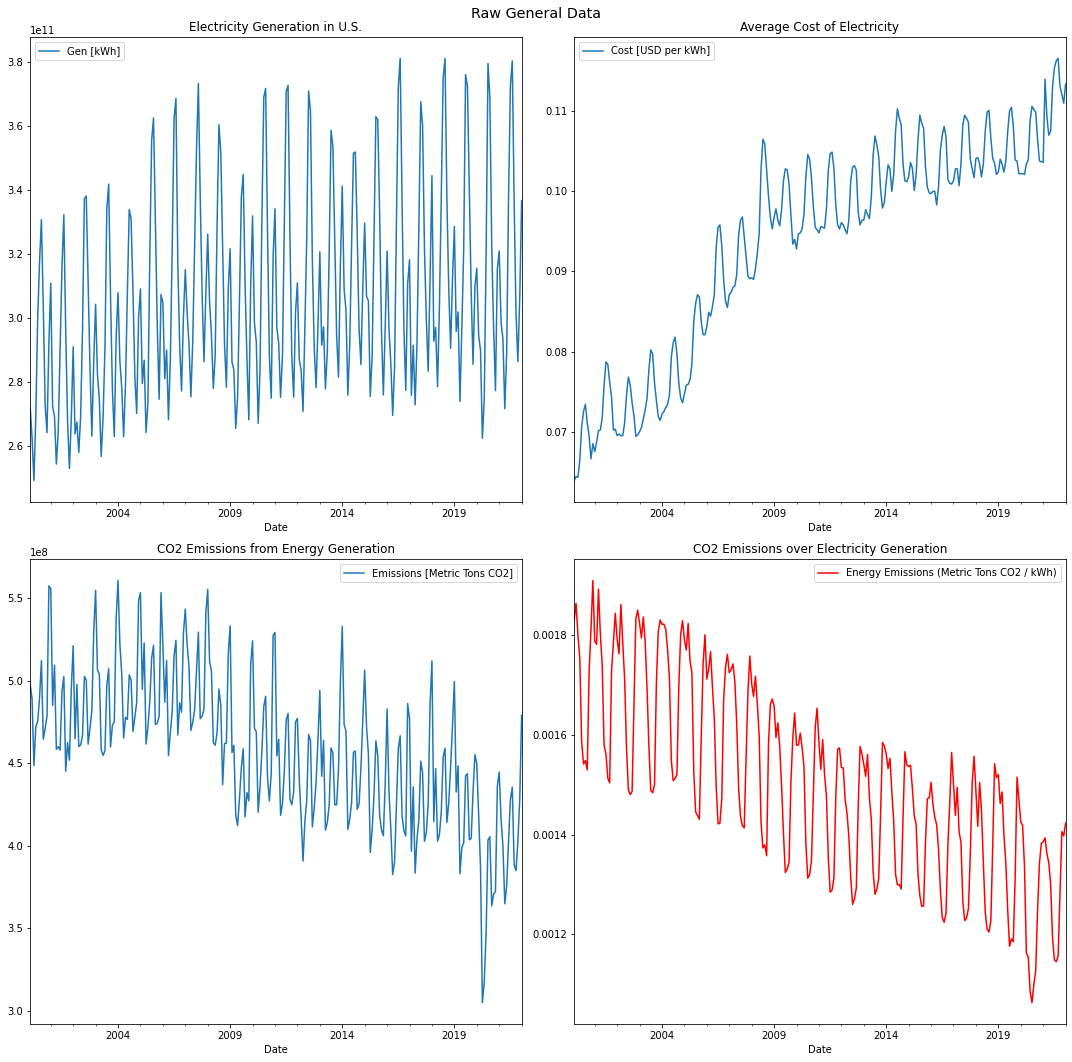
\includegraphics[width=\linewidth]{images/us_energy_data.png}
    \caption{Graphs depicting electricity generation over time, electricity cost over time, $\text{CO}_2$ emissions over time, and $\text{CO}_2$ emissions (in metric tons) per kWh of generated electricity over time. }
    \label{fig:us_data}
\end{figure}

This initial step revealed that the cost of electricity in the U.S. has increased over time, while the amount of $\text{CO}_2$ emitted from electricity generation has decreased over time. This is not particularly surprising, as certain regions within the U.S. have recently been converting to cleaner sources of electricity \cite{clean_energy}.

After collecting general energy-related data, we moved on to collecting coin-specific data. Data was collected for each of the cryptocurrencies described in the ``Coins'' section of this report (with the exception of SolarCoin).

For each coin, we were interested in several metrics, including price over time, average amount of energy required for each transaction, and the average number of transactions performed per day. Using this data and the U.S. energy data collected previously, we were able to make several important computations. We first determined the amount of money (in USD) spent on energy over time for each coin's transactions (Fig. \ref{fig:cost_per_tx}). 

\begin{figure}[h!]
  \centering
  \begin{subfigure}[b]{0.5\linewidth}
    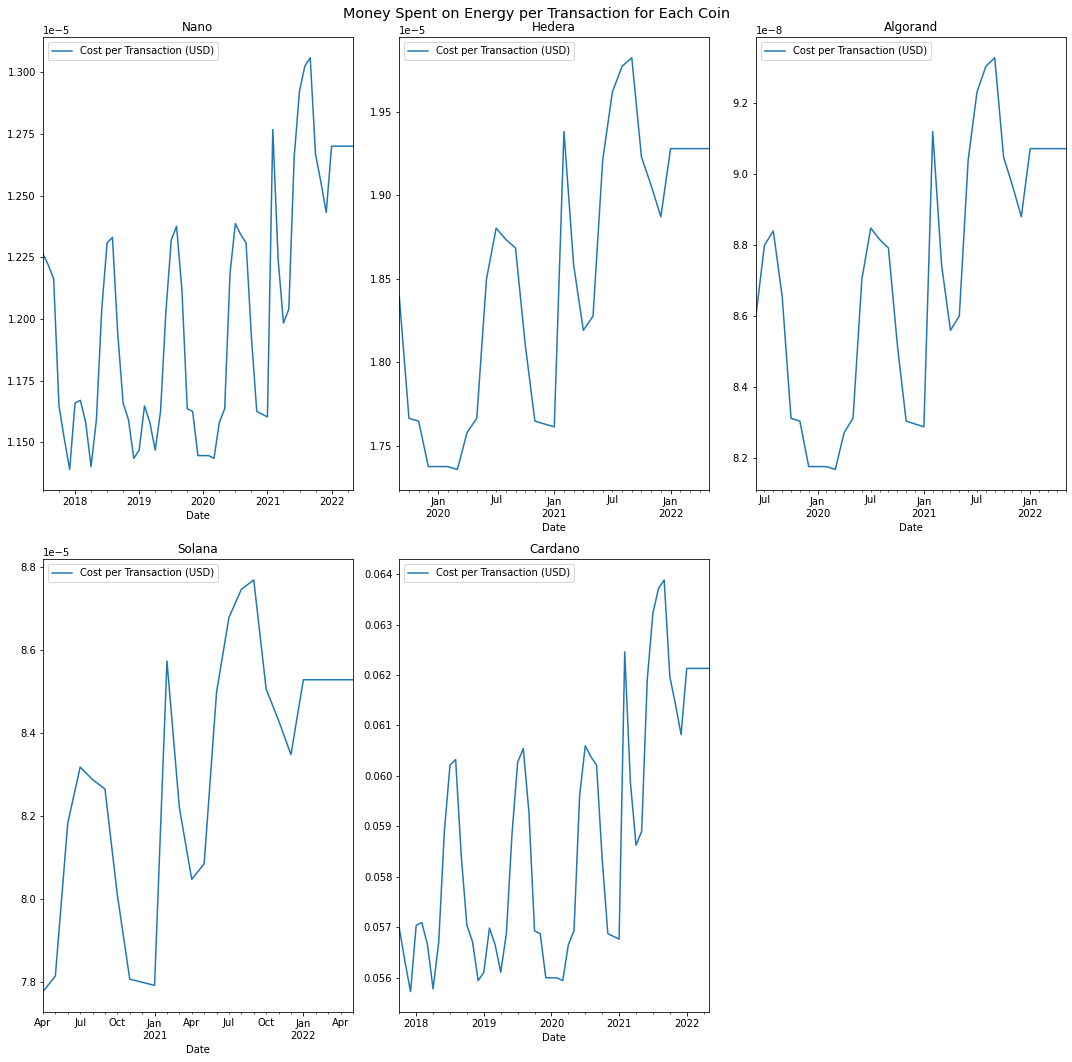
\includegraphics[width=\linewidth]{images/money_on_energy_per_transaction.png}
    \caption{Cost of energy required to complete a transaction over time for each coin.}
  \end{subfigure}
  \begin{subfigure}[b]{0.45\linewidth}
    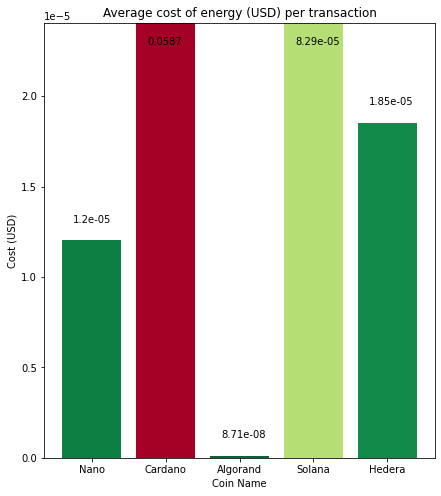
\includegraphics[width=\linewidth]{images/average_cost_per_transaction.png}
    \caption{Average cost of energy for a transaction for each coin.}
  \end{subfigure}
  \caption{Cost of energy for each coin's transactions.}
  \label{fig:cost_per_tx}
\end{figure}

We then performed a similar analysis to determine the quantity of carbon dioxide ($\text{CO}_2$) emissions generated by the production of energy needed to perform each coin's transactions (Fig. \ref{fig:co2_per_tx}).

\begin{figure}[h!]
  \centering
  \begin{subfigure}[b]{0.5\linewidth}
    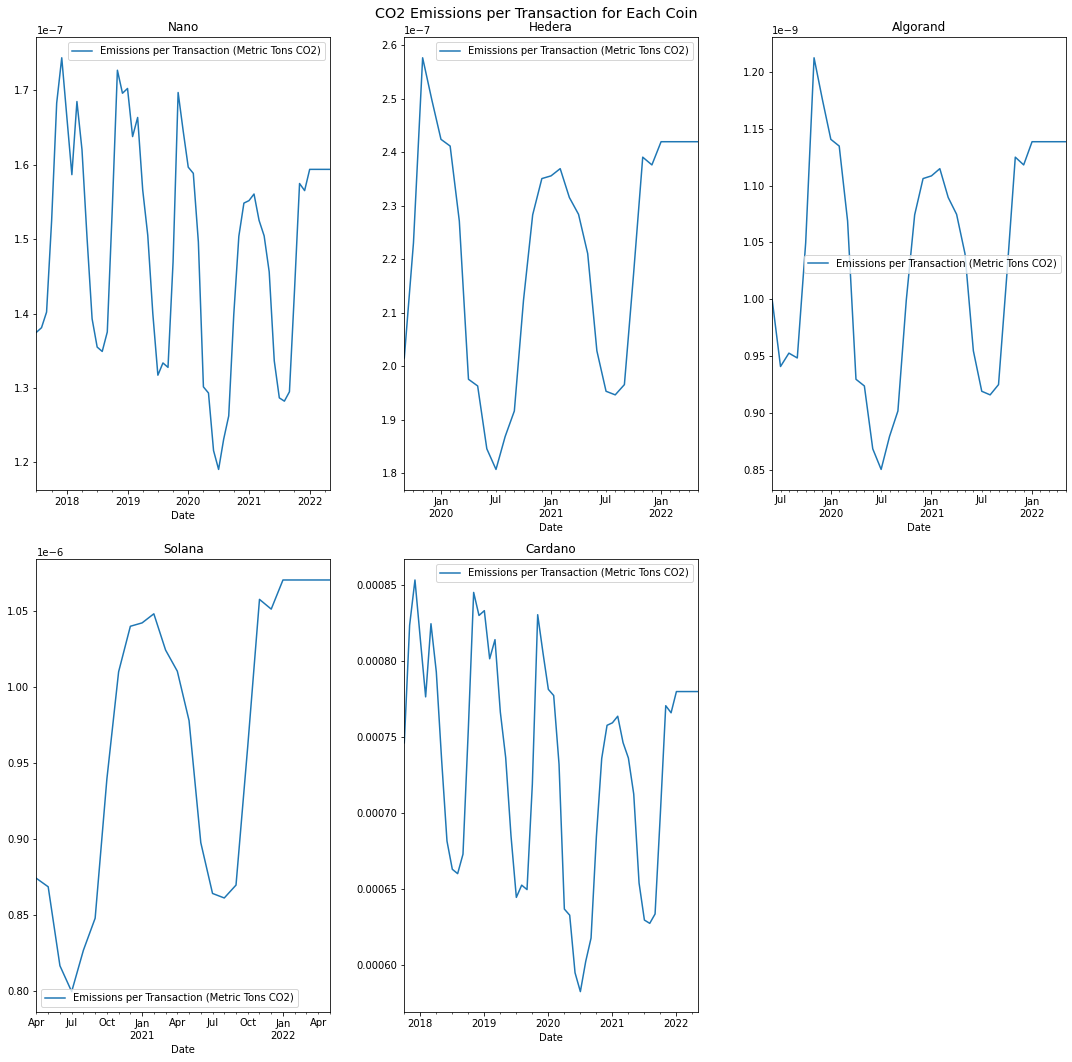
\includegraphics[width=\linewidth]{images/emissions_per_transaction.png}
    \caption{$\text{CO}_2$ emissions from energy production per transaction over time for each coin.}
  \end{subfigure}
  \begin{subfigure}[b]{0.45\linewidth}
    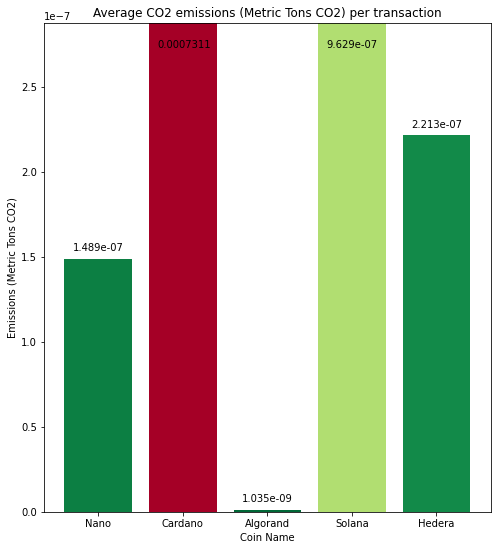
\includegraphics[width=\linewidth]{images/average_emissions_per_transaction.png}
    \caption{Average emissions due to energy production for a transaction for each coin.}
  \end{subfigure}
  \caption{$\text{CO}_2$ emissions from energy production for each coin's transactions.}
  \label{fig:co2_per_tx}
\end{figure}

Then we computed the climate-related societal damages caused by completing one transaction for each coin. After this step, we had all of the information required to compute the net social value for each coin over time (Fig. \ref{fig:net_social_value}). 

\begin{figure}[h!]
    \centering
    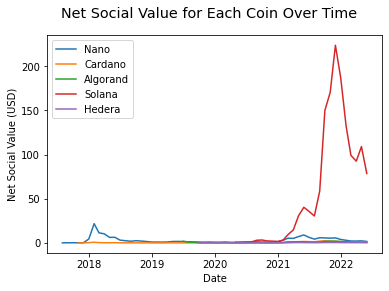
\includegraphics[width=\linewidth]{images/net_social_value_over_time.png}
    \caption{Net social value of each coin over time. }
    \label{fig:net_social_value}
\end{figure}

\begin{figure}[h!]
  \centering
  \begin{subfigure}[b]{0.45\linewidth}
    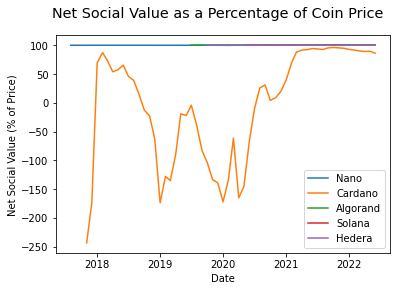
\includegraphics[width=\linewidth]{images/net_social_value_percent.png}
  \end{subfigure}
  \begin{subfigure}[b]{0.45\linewidth}
    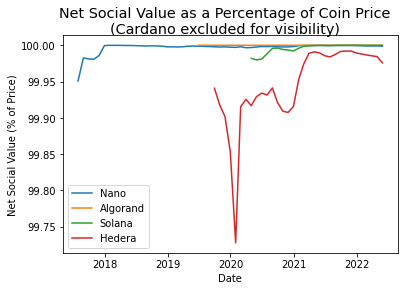
\includegraphics[width=\linewidth]{images/net_social_value_percent_no_cardano.png}
  \end{subfigure}
  \caption{Net social value of each coin over time as a percentage of that coin's price.}
  \label{fig:net_social_value_percents}
\end{figure}

\section{Assessment}

As seen on the graph for net social value of each coin over time (Fig. \ref{fig:net_social_value}), Solana has a much higher net social value than the other coins. It achieves this despite its relatively high emissions per transaction because of its much higher price. The high market price of the coin is enough to offset these social damages to result in a very positive net social value. This indicates that Solana is a great short-term alternative to the dominant POW coins like BitCoin and Ethereum 1.0- it clearly has high demand in the cryptocurrency market, and has much greater net social value due to the extreme resources required with POW models.

However, as we know, the price of cryptocurrencies fluctuate heavily. Prices may often be driven around hype, and it is difficult to predict what cryptocurrencies will look like in a few years because they are so new. Though Solana has a high price at the moment compared to the other coins, that may not be the case in the future. Instead, if we looked more at metrics that were less susceptible to fluctuation - such as energy per transaction - other cryptocurrencies begin to look more favorable. 

The graphs in Figure \ref{fig:net_social_value_percents} can give some insight into a less price-biased metric, as they depict the net social value of each coin as a percentage of the coin's price over time. These charts do indeed show that Algorand, Nano and Solana have consistently high net social value compared to the other coins in the study.

Algorand in particular performs transactions with far lower cost and climate-related damages compared to the other coins discussed. It averages $1.035 * 10^{-9}$ metric tons of carbon dioxide emission per transaction; the next lowest is Nano at $1.489 * 10^{-7}$. In addition, Algorand is currently seeing a period of hyper-growth, indicating that the price could be much higher in the future. If this is the case, Algorand could certainly be an incredible green alternative to dominant POW coins. 

The metrics obtained for Algorand's energy per transaction is a theoretical amount. If we were to no longer consider Algorand because of this, the other most appealing coins in terms of cost per transaction and emission produced are Nano and Hedera. Nano specifically has the potential to fulfill the role of BitCoin with much better speeds, transaction amounts, and energy usage. BitCoin, however, is a currently an insurmountable giant in the cryptocurrency market when it comes to scale and capital. 

\section{Limitations}

There were a number of limitations that were encountered when trying to gather data for this paper. Many of them were due to the fact that the coins that were researched are less popular than those from the Goodkind paper, and thus have less publicly available data.

Not only were the coins less popular, but our research also focused on Proof-Of-Stake protocols. Because consensus methods in POS require negligible energy compared to mining with POW, the data for the consensus method energy requirements was not something we could easily find. Additionally, the energy required for transactions was the data that was more widely available and advertised, so this metric is what we focused on for the POS coins.

The scope of our analysis was also affected by the limitation of data. Specifically, we would ideally be able to find data for the energy required per transaction as well as the number of transactions per day over time. We were unable to find any data that reported the change in these metrics. The energy required per transaction is not something that should scale too heavily with a POS model, but transaction frequency is certainly something that would grow heavily as the coin gained popularity, and thus would affect the energy the blockchain requires. Because we were not able to find this data as a time series, we had to resort to assuming constant values for transaction frequency and energy required per transaction.

The analysis of Algorand was based off of a theoretical foundation of all validators having the same, highly efficient hardware (Raspberry PI). And assuming a transaction rate of 1000 transactions per second. Since Algorand is regarded as on of the greenest coins, we wanted to evaluate the theoretical potential of one of these systems, despite not using the full data.

Additionally, the Goodkind paper considered the health effects caused by energy-related emissions in their calculations for social damages. This is something we would have liked to include, however we did not have access to this data. Instead, we focused on the societal costs of carbon dioxide emissions as this data was readily available and accessible.

\section{Conclusion}

Cryptocurrencies have the potential to change the way the world economy is maintained, but they must be better researched and improved upon to a more sustainable system, such that we do not use too much energy for maintenance of the financial system and potentially harm the environment and contribute to global warming. 

POS systems seem to resolve at least some of the issues of scalability that POW systems cannot overcome. The trade-off is that we must now pay the price of an opportunity cost on the money we stake in order to maintain the system. Despite this, it is evident that POS systems require much less energy for maintenance, even in examples of increased popularity (Solana, Algorand, & Cardano), the POS coins did not exceed $0.6$ kWh per transaction, while Ethereum uses $240$ kWh per transaction, and BitCoin towers at $1,173$ kWh per transaction. Mass adoption of these POS coins has not yet been realized, but innovations like this will help drive the mass adoption of cryptocurrencies in general, as they become more sustainable and practical.

With further research we could see a coin that has all of the desirable characteristics of a dominant currency with the potential to become the world reserve currency.

\pagebreak
\section{Contributions}
\subsection{Taylor Giles}
\begin{itemize}
    \item Analysis and data collection for Hedera
    \item Analysis of SolarCoin
    \item U.S. energy \& emissions data collection
    \item Data cleaning and visualizations
    \item Report ``Procedure \& Data Collection'' section
\end{itemize}

\subsection{Matthew Broadbent}
\begin{itemize}
    \item Analysis and data collection for Nano
    \item Analysis and data collection for Cardano
    \item Report ``Assessment'' section
    \item Report ``Limitations'' section
    \item Report ``Introduction'' section
\end{itemize}

\subsection{Srdjan Bozin}
\begin{itemize}
    \item Analysis and data collection for Algorand
    \item Analysis and data collection for Solana
    \item Report ``Conclusion'' section
    \item Report ``Limitations'' section
    \item Report ``Introduction'' section
\end{itemize}

\pagebreak

\printbibliography

\noindent
Data and processing code can be found at: \\ \url{https://github.com/taylor-giles-sbu/CSE551-Final-Project}

\end{document}
